\chapter{Theoretical Framework}

This chapter reviews the actual state and the basis of the e-learning, as well as the theoretical base to model ultrashort-pulse propagation in fibers. Spectral and time broadening are fundamental aspects of nonlinear fiber optics. Understanding their basis and how they affect the propagation of an electromagnetic wave is an essential factor to both develop the code and test its effectiveness. Providing an overview of the equations describing the light propagation in a dispersive, nonlinear medium gives the principles to see what is solved with the back-end code at further stages in this thesis project.




\section{Background: Constructivism and other theories of education}
This section aims to review some of the existing theories about interactive learning and how to enhance the experience of the students. Some projects presented help to the construction and planning of the final product desired: a web-oriented code modeling the propagation of ultrashort pulses in optical fiber.



\subsection{Constructivism}
Constructivism is a theory of cognition that proposes using unconventional instruction methods to fulfill the ever-active process of learning, this while not ignoring the idea that students are individuals who may perceive the learning environment in a different way than how the teachers intend to present it. Moreover, according to \cite{fosnot2013constructivism}, "the task of the educator is not to dispense knowledge but to provide students with opportunities and incentives to build it up;" that means adapting to the diverse forms of thinking, instead of assuming that the students will acquire this knowledge just from the means already given to them.


\subsection{E-Learning}
The increasing quantity of online, partially online, or presential courses with strong online interactions strives to supply the necessity from a generation of students (with a strong influence of technology and social networks) to incorporate E-Learning in the teaching methods and the learning environments.  According to \cite{vltool}: "interactivity is a key feature of online education which helps attract and retain students in online classes," thus applying visual learning tools together with an online learning experience can develop engagement and motivation in the learning process in students. 

One can refer then to E-Learning as "the use of both software-based and online learning"  \cite{tabak} and, according to \cite{tabak}, \cite{munoz}, it has to be flexible, accessible, and intuitive. Hence factors like clear instructions, the relevance of the topics, the requirements to use its tools, and the difficulty to use them are crucial to implementing E-learning in different courses for different levels of education.

\section{Background: Interactive Learning tools}

Enhancing the students' learning experience regardless of the education level can be achieved using different interactive E-Learning tools, e.g., Web sites like Mathweb or mobile apps like I-MMAAPS. The interface of the interactive and personalizable content of these tools is essential to create a successful and effective tool \cite{vltool}. Therefore it should also be taken into account while creating an interactive E-Learning tool. Chapters 1 and 2 discuss how the interface was designed  and how a group of students perceived it.\textbf{ (give more details at the end of the project). }



\subsection{examples of Interactive Learning tools}
To know more about interactive learning is imperative to look at previous works and how they can contribute to the creation of new tools like the one discussed in this thesis.

\subsubsection{Mathweb}
The Hochschule Ruhr West has developed a website named \href{https://mathweb.de/}{"Mathweb"}   to support the students during the semester and preparation for the exams. According to surveys,  students underestimate the continuous study (during and after evaluations), among other problems related to learning strategies, that led to the endorsement of this Web amongst the students who, after the trial period, see it as a helpful tool and perceive a positive impact in their studies \cite{MathWeb}.

On this website are available a wide variety of examples, interactive demonstrations with graphics, explanations, exercises, and the option to check if the solution given by the user is correct. The themes included going from simple mathematical operations to more complex topics like derivatives are available for everyone, even though the test course cannot be accessed signed in as a guest.

\subsubsection{I-IMAPPS}

I-IMAPPS is an application created at the Universiti Teknologi MARA Sarawak in Malaysia and aimed to promote the learning of the indigenous Iban language using situations immerse in possible environments where its use is necessary. The researchers worked based on constructivism and the premise that mobile learning is an alternative to study a language if the people do not have the time for intensive or immersive lessons. 


To develop and structure this app, they followed the ADDIE Model, which consists of five aspects: 

\begin{enumerate}
    \item Analysis: gathering and selecting the information, phrases, and vocabulary of the Iban language; investigation on the availability (if there are existing apps created for this purpose, which is not the case) and focus on the learning objectives of the mobile app.
    \item Design: description of the message to send and the user interaction with the content, layout, and storyboard design focused on the cultural aspects of this language. The content framework comprehends the resources (multimedia elements like text, audio animations, etc.), learning theories allowing the user to work autonomously, and interactivity.
    
    \item Development: the researchers used Flash for the animations, Photoshop CS5  for the illustrations, and Corona SDK for software engineering. 

    
    \item Implementation.
    
    \item Evaluation: 30 non-native speakers tested the I-MMAPPS prototypes, did a test of the new knowledge obtained, and gave feedback on the experience using them.
    
\end{enumerate}

The conclusion of this research points that this app helps developing interest and assists non-native speakers at the early stages of learning this language. Further work needs to be done to improve the app's features \cite{CHACHIL2015267}. 



\subsubsection{Control courses}
Björn Wittenmark, Helena Haglund, and Mikael Johansson at Lund Institute of Technology used interactive learning and dynamic pictures to aid the students while learning abstract parts of the theory in control courses. The goal was not just to have students with a solid theoretical understanding of the topics but also to have high engineering capabilities; this relies on the good connection of the theory by improving the comprehension of the students and the practical aspect of the problems presented. One way to achieve this is with material available "anywhere and anytime" using the web and Matlab and Simulink for the computations. 

They implemented dynamic pictures where the user can see the effect of, e.g., changing a parameter in continuous-time poles and zeroes plots without typing commands. Drags, dropdowns, text input slots, and buttons enhance the graphical interface of the CCSDEMO. This tool makes active learning possible covering topics like robustness, tuning of PID-controllers, observability, among other subjects of the 13 available modules. They highlight the idea that it is meaningful to design the interface carefully to allow an intuitive use avoiding the need to read a manual and contributing to the utilization without supervision.

In conclusion, dynamic pictures improve the courses giving the students more tools than just pre-canned video or static data and illustrations, motivating the students who responded encouragingly \cite{IEEEcontrol}.




\section{Eigenvalue problem}

    \subsection{Planar Waveguide}
        
        
        
        \begin{figure}[label={fig_planarwave}, caption={Sketch of a planar waveguide.}]
          %  \caption*{Source: Some Source}
                \centering  
                \tikzset{every picture/.style={line width=0.75pt}} %set default line width to 0.75pt   
        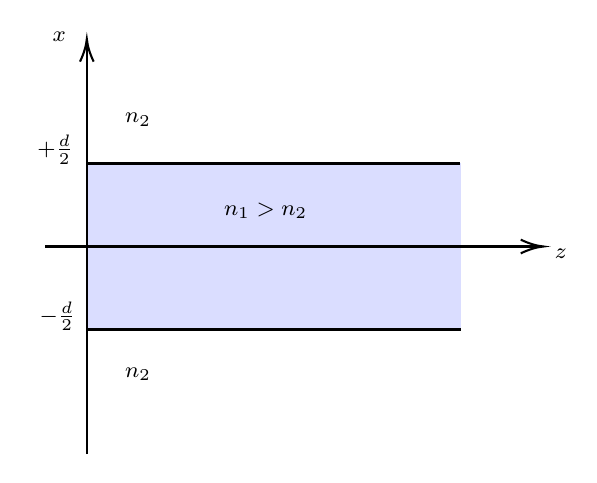
\begin{tikzpicture}[x=0.75pt,y=0.75pt,yscale=-1,xscale=1]
        %uncomment if require: \path (0,310); %set diagram left start at 0, and has height of 310
        
        %Shape: Rectangle [id:dp439999456910388] 
        \draw  [draw opacity=0][fill={rgb, 255:red, 218; green, 221; blue, 255 }  ,fill opacity=1 ] (100,80) -- (280.5,80) -- (280.5,160) -- (100,160) -- cycle ;
        %Shape: Boxed Line [id:dp5082075899729874] 
        \draw    (80,120) -- (318,120) ;
        \draw [shift={(320,120)}, rotate = 180] [color={rgb, 255:red, 0; green, 0; blue, 0 }  ][line width=0.75]    (10.93,-3.29) .. controls (6.95,-1.4) and (3.31,-0.3) .. (0,0) .. controls (3.31,0.3) and (6.95,1.4) .. (10.93,3.29)   ;
        %Shape: Boxed Line [id:dp5101173446407539] 
        \draw    (100,220) -- (100,22) ;
        \draw [shift={(100,20)}, rotate = 450] [color={rgb, 255:red, 0; green, 0; blue, 0 }  ][line width=0.75]    (10.93,-3.29) .. controls (6.95,-1.4) and (3.31,-0.3) .. (0,0) .. controls (3.31,0.3) and (6.95,1.4) .. (10.93,3.29)   ;
        %Shape: Boxed Line [id:dp2709424820833741] 
        \draw    (100.5,160) -- (280.5,160) ;
        %Shape: Boxed Line [id:dp10541842748284669] 
        \draw    (100,80) -- (280,80) ;
        
        
        % Text Node
        \draw (74.67,64.73) node [anchor=north west][inner sep=0.75pt]  [font=\footnotesize]  {$+\frac{d}{2}$};
        % Text Node
        \draw (72,145.07) node [anchor=north west][inner sep=0.75pt]  [font=\footnotesize]  {$\ -\frac{d}{2}$};
        % Text Node
        \draw (164.67,97.73) node [anchor=north west][inner sep=0.75pt]  [font=\footnotesize]  {$n_{1}  >n_{2}$};
        % Text Node
        \draw (117,177.07) node [anchor=north west][inner sep=0.75pt]  [font=\footnotesize]  {$n_{2}$};
        % Text Node
        \draw (117,54.4) node [anchor=north west][inner sep=0.75pt]  [font=\footnotesize]  {$n_{2}$};
        % Text Node
        \draw (324,119.73) node [anchor=north west][inner sep=0.75pt]  [font=\footnotesize]  {$z$};
        % Text Node
        \draw (82,15.07) node [anchor=north west][inner sep=0.75pt]  [font=\footnotesize]  {$x$};
        
        
        \end{tikzpicture}
        
        \end{figure}
          
        Figure \ref{fig_planarwave} shows a planar waveguide consisting of two materials with refractive indices $n_1$ for the core and $n_2$ for the cladding. This waveguide is infinite in the y-direction, has a thickness $d$ (which satisfies that $d >> \lambda$), and fulfills the total internal reflection condition at the boundary \citep{yariv_b}, \citep{OKAMOTO200613}.  Its transverse propagation constant is
        
        
                    \begin{equation}
                        h=\sqrt{k_0^2n_1^2-\beta^2},
                        \label{eq_h}
                    \end{equation}
         where $\beta$ and $h$ are for the core region. For the cladding region, we have the longitudinal propagation constant $\kappa$
        
                     \begin{equation}
                        \kappa=\sqrt{\beta^2-k_0^2n_2^2}.
                        \label{gam}
                    \end{equation}
         
         Here $k_0 = \omega_0/c$ is the wavenumber in vacuum.
        
        
        
        We can include U, W, and V
        
                    \begin{equation}
                        U^2+W^2 = V^2 = k_0^2a^2(n_1^2-n_2^2) \
                        \begin{cases}
                            U = a \times h \\
                            W = a \times \kappa
                        \end{cases} 
                        \label{Normv},
                    \end{equation}
        where V is the so-called waveguide parameter or normalized frequency. 
        The TE mode is then given by 
                 
                    
                    \begin{equation}
                    \textbf{TE mode} \ \ W=
                        \begin{cases}
                            U \tan(U) & \text{even mode}\\
                            -U cotan(U) & \text{odd mode}
                        \end{cases}
                        \label{Temode}
                    \end{equation}
        
        We can solve the eigenvalue problem graphically by plotting W as a function of U [Joly's lecture]. Figure \ref{fig:eigen1} shows this approach where the circle has a radius of V.
        
        
        \begin{figure}[label={fig:eigen1}, caption={Visualization of the graphic solution of the eigenvalue problem. Taken from \cite{herokuapp}}]
          %  \caption*{Source: Some Source}
        	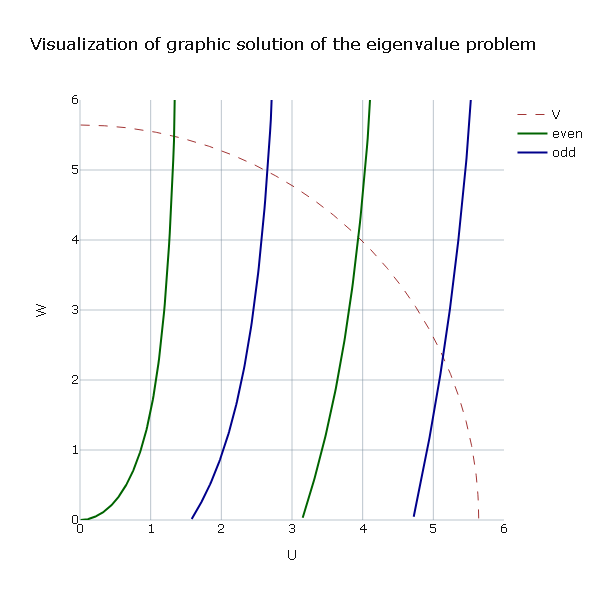
\includegraphics[width=.6\textwidth]{figures/chap2/Eigenvalue.png} 
        \end{figure}
        
        We created a code at the Max-Plank institute \cite{gitmax} to show the students how a change of parameters can affect the plot and, thus, the solutions of the eigenvalue problem. This web tool aims to help the students understanding this problem, and figure \ref{fig:planarp}  shows the interface. The code is written in Python and the Web interface made with Dash/Plotly.  
        
        \begin{figure}[label={fig:planarp}, caption={\href{https://fiber-mode-app.herokuapp.com/apps/dash_plot}{Heroku app} for the planar waveguide.}]
          %  \caption*{Source: Some Source}
        	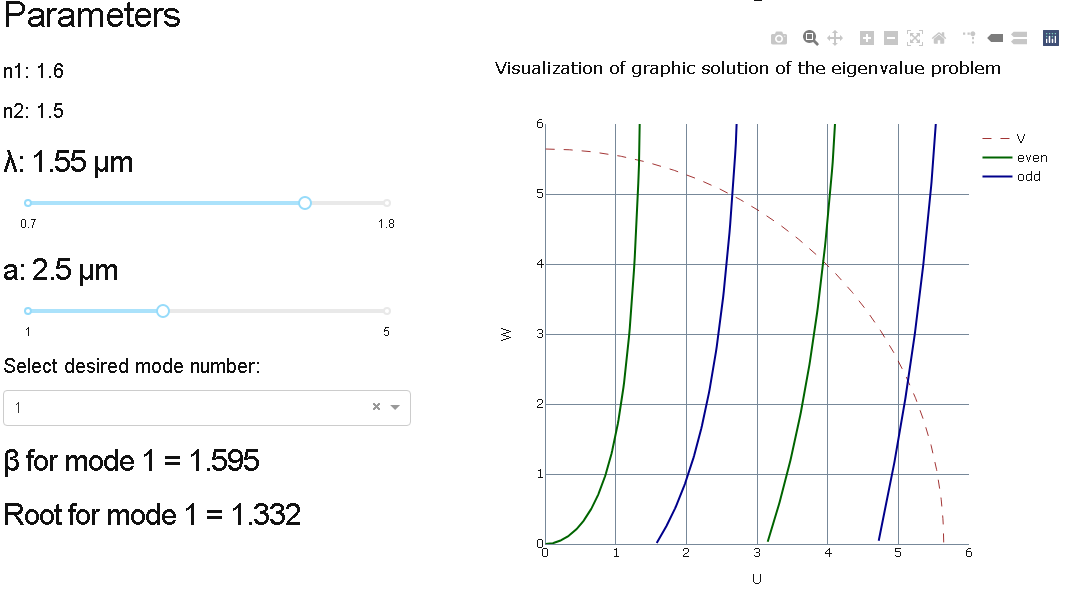
\includegraphics[width=.8\textwidth]{figures/chap2/planarpage.png} 
        \end{figure}
        
        
        Heroku is a web that supports programming languages like Java, Node.js, Python, among others \cite{heorku}. The codes for the planar waveguide and the optical fiber were deployed using its free service.

    \subsection{Optical Fiber}
    
        The code can also solve the problem for the optical fiber, and the students can change some more parameters like cladding and core material, see the Poynting vector or some of the cuts of the field. Figures \ref{fig:fibre1} and \ref{fig:fibre2} show this web. 
        
        
        The refractive index of a material can be approximated by 
        \begin{equation}
            n^2 (\omega) = 1 + \sum_{j=1}^{m} \frac{B_j\omega^2_j}{\omega^2_j - \omega^2} 
            \label{eq_ene}
        \end{equation}
        called the Sellmeier equation. Here $\omega_j$ is the resonance frequency and $B_j$ the strength of it \citep{AgrawalBook}. This allowed to add the different materials to de code an can be changed by selecting the material in the dropwdowns for the core and the cladding of the fiber.
        
        
        \begin{figure}[label={fig:fibre1}, caption={\href{https://fiber-mode-app.herokuapp.com/apps/results}{Heroku app} for the optical fiber (1).}]
          %  \caption*{Source: Some Source}
        	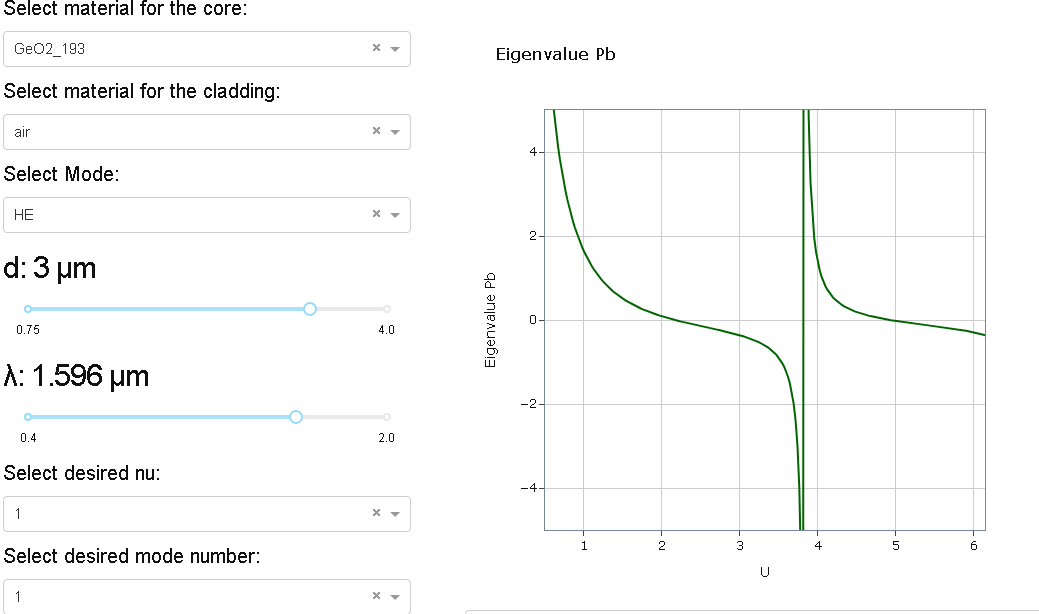
\includegraphics[width=.8\textwidth]{figures/chap2/fibre1.PNG} 
        \end{figure}
        
        \begin{figure}[label={fig:fibre2}, caption={\href{https://fiber-mode-app.herokuapp.com/apps/results}{Heroku app} for the optical fiber (2).}]
          %  \caption*{Source: Some Source}
        	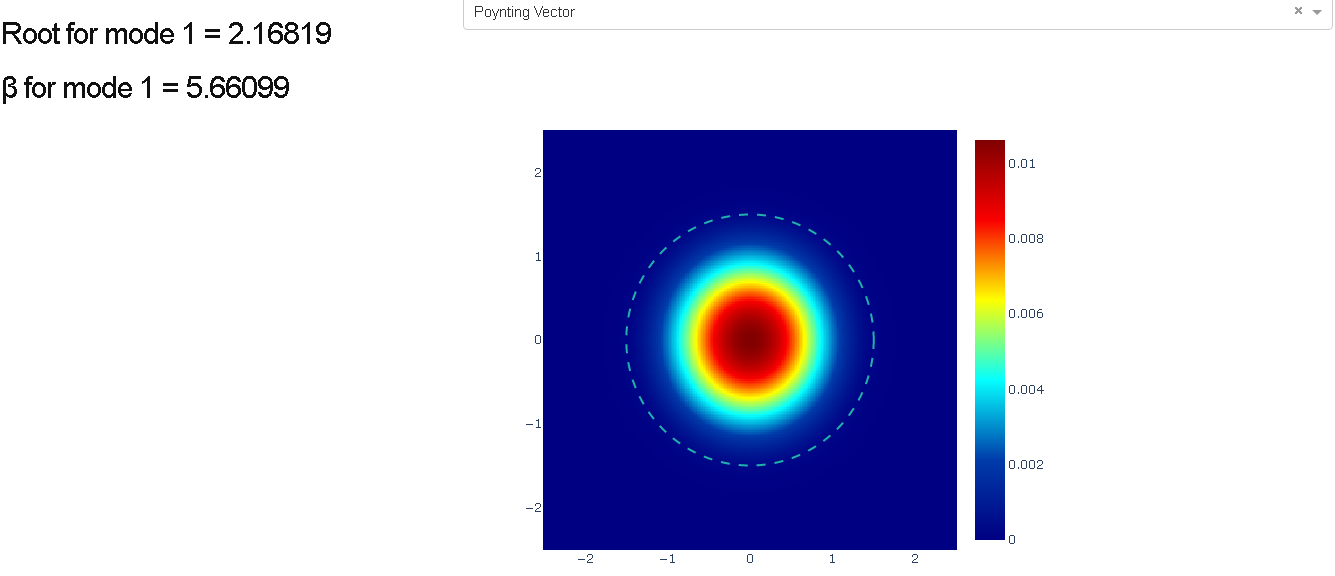
\includegraphics[width=.8\textwidth]{figures/chap2/fibre2.PNG} 
        \end{figure}
    

   


\section{Pulse propagation in fibers}

Loss and dispersion originated by interactions of the electromagnetic field with the atoms of the medium, and frequency dependence of the refractive index affect the propagation of an electromagnetic wave through this medium \citep{dudley_taylor_2010}. Shape and spectrum of short pulses with widths between approx. 10ns and 10fs propagating in a fiber are affected by nonlinear and dispersive effects \citep{AgrawalBook}.  

    \subsection{Pulse evolution inside a single-mode fiber:}
        The slowly varying amplitude \emph{A(z,t)} can be described by the equation:
        \begin{equation}\label{eq_a}
        \begin{split}
            \frac{\partial A}{\partial z}&= \overbrace{-\frac{\alpha}{2} - \beta_1\frac{\partial A}{\partial t} - \frac{i \beta_2}{2} \frac{\partial^2 A}{\partial t^2} +\frac{\beta_3}{6} \frac{\partial^3 A}{\partial t^3}}^{\mathbf{linear \ effects}}\\  
            & +\underbrace{i \gamma \left( 1 + \frac{i}{\omega_0} \frac{\partial}{\partial t} \right) \left( A(z,t) \int_{-\infty}^{\infty} R(t') \left|A(z, t-t') \right|^2 \ dt'  \right)}_{\mathbf{nonlinear \ effects}}
        \end{split}
        \end{equation}
    %[A] = sqrt(W)
    where: 
    \begin{itemize}
        \item \textbf{t} is the time variable [s]
        \item \textbf{z} is the space variable [m]
        \item $\mathbf{\alpha}$ is the attenuation coefficient [1/m]
        \item $\mathbf{\beta_n}$ are propagation constant coefficients $[s^n/m]$
        \item $\mathbf{\gamma}$ is the nonlinear parameter [1/Wm]
        
            \begin{equation}
                \gamma = \frac{n_2 \omega_0}{c A_{eff}},
                \label{eq_gamma}
            \end{equation}
        with $\mathbf{n_2} \quad [m^2/W]$ which is the nonlinear refractive index, and $A_{eff} \quad [m^2]$ that  is the  effective core area.
        %or  n2 is the nonlinear-index coefficient. 
        \item \textbf{R(t)} [1/s] is the response function that includes electronic and vibrational contributions and is approximated by 
        
        \begin{equation}\label{eq_rt}
            R(t) = (1- f_R)\delta(t) + f_R h_R(t),
        \end{equation}
        where $f_R$ and $h_R(t)$ are the fractional contribution of the delayed Raman response and the Raman response function, respectively. Conforming to \cite{dudley_taylor_2010}, 
        \begin{equation}\label{eq_hr}
            h_R(t) = \frac{\tau^2_1+\tau^2_2}{\tau_1\tau^2_2} exp(-t/\tau_2)sin(t/\tau_1)\Theta(t),
        \end{equation}
        here $\delta(t)$ and $\Theta(t)$ are the Delta Dirac and the Heaviside step functions, respectively; $f_R = 0.18$,  $\tau_1 =12.2 fs$, and $\tau_2 = 32 fs$.
         
         
        \item $\omega_0$  is the center angular frequency
    
    \end{itemize}
   
    One can asume that the evolution of the envelope pulse is slow, and remembering that the group velocity is defined by 
    
    \begin{equation}\label{eq_vg}
        v_g \equiv \frac{1}{\beta_1}, 
    \end{equation}
    and the pulse can be moved at the group velocity using the reference frame 
    \begin{equation}\label{eq_t}
        T = t - \frac{z}{v_g}. 
    \end{equation}
    
    Thus, equation \eqref{eq_a} can be defined as 
    
    \begin{equation}\label{eq_b}
        \frac{\partial A}{\partial z}=-\frac{\alpha}{2} - \frac{i \beta_2}{2}A \frac{\partial^2 A}{\partial T^2} +\frac{\beta_3}{6} \frac{\partial^3 A}{\partial T^3} +i \gamma   \left(A\left|A\right|^2+ \frac{i}{\omega_0} \frac{\partial}{\partial T} (A\left|A \right|^2)- A \ T_R \frac{\partial \left|A \right|^2}{\partial T} \right),
        \end{equation}
    where the first moment of the nonlinear (Raman) response is
    \begin{equation}\label{eq_TR}
        T_R = f_R\int_{0}^{\infty} t \ h_R(t) \ dt.
    \end{equation}

        
    \subsection{NLSE}
        According to \citep{AgrawalBook}, the equation  \eqref{eq_b} for the slowly varying envelope can be simplified for pulses of width $T_0 > 5 ps$ to
        \begin{equation}
                \frac{\partial A}{\partial z} = -\frac{\alpha}{2}A-j \frac{\beta_2}{2}\frac{\partial^2A}{\partial T^2}+j\gamma|A|^2 A,
                \label{eq_nlse}
            \end{equation}
            \ \\
       It is noteworthy that the contribution of the third-dispersion term should be considered if $\beta_2 \approx 0$ (zero-dispersion region). Equation \eqref{eq_nlse} is known as the nonlinear Schrödinger equation (NLSE).

           Following the convention used in \cite{AgrawalBook}, \cite{dudley_taylor_2010} , the continuous inverse Fourier transform of the slowly varying function of z is
        
        \begin{equation}\label{eq_acft}
            A(z,t) = \frac{1}{2\pi} \int_{-\infty}^{\infty} %\tilde{A}(z,\omega-\omega_0)\exp{[-i(\omega-
            \tilde{A}(z,\omega)exp(-i\omega t) \ d\omega \ .
        \end{equation}
        
        
        The FFT is an algorithm capable of calculating the discrete Fourier transform faster \citep{Lynch2018}. The definition of \href{https://numpy.org/doc/stable/index.html}{Numpy} of the inverse DFT as \cite{dft} says is 
        \begin{equation}\label{eq_dft}
            a_n = \frac{1}{n}\sum_{k=0}^{n-1} A_k \ exp\left\{ 2\pi i \frac{mk}{n} \right\} \qquad m = 0,...,n-1,
        \end{equation}

        then, it follows
        \begin{equation} \label{eq_deffft}
                A(z,T) = FFT \left[ \tilde{A}(z,\omega) \right].
            \end{equation}
            
            
    \subsection{Dispersion}
        The frequency dependency of the refractive index can lead to different speeds of propagation from different wavelengths of pulses in a fiber, which causes a broadening of the pulse in the time domain. This effect can limit the transmission of information and generate effects like inter symbol interference.  So, one can call chromatic dispersion the delay between several spectral components of a traveling pulse, i.e., there are different group velocities for the diverse components propagating in the fiber  \citep{Udayakumar2013ChromaticDC}. This delay depends on the waveguide (e.g., core radius) and material (e.g., the difference between core and cladding indices) contributions \citep{dudley_taylor_2010}. 
        
        The Taylor series expansion of the propagation constant 
        \begin{equation}
             \beta(\omega) = n (\omega)\frac{\omega}{c} = \beta_0 + \beta_1(\omega-\omega_0) \frac{1}{2}\beta_2(\omega-\omega_0)^2+...\, 
             \label{eq_betas}
        \end{equation}
        with 
        \begin{equation}
            \beta_m = \frac{d^m\beta}{d\omega^2}_{\omega = \omega_0} \qquad (m = 0,1,2,...),
            \label{eq_dbeta}
        \end{equation}
        
        
        defines the Group Velocity Dispersion (GVD) parameter $\beta_2$  and higher-order dispersion terms.  $\beta_2$ is also related to the dispersion parameter D by
        \begin{equation}
            D = \frac{d\beta_1}{d\lambda} = - \frac{2\pi c}{\lambda^2}\beta_2 \quad [\frac{ps}{nm \ km}] \ .
            \label{eq_Ds}
        \end{equation}
        
        Depending on the value of the GVD parameter, either shows the fiber a normal dispersion ($\beta_2 > 0$ , $D<0$), or it is in the anomalous dispersion regime ($\beta_2 < 0$ , $D>0$).
        
        Linear solitons can reduce this effect, even though there are several methods to compensate chromatic dispersion, as \cite{AgrawalBook}, \cite{dudley_taylor_2010},  and \citep{Udayakumar2013ChromaticDC} explain. Dispersion compensating fiber (DCF), Fiber Bragg Grating (FBG), and Optical Phase Conjugator (OPC) are some of the methods used.
        
       

    \subsection{Nonlinear Effects}

        Nonlinearities can be effects such as third-harmonic generation, four-wave mixing (FWM). The Kerr nonlinearity $n = n(P_{opt})$
        can lead to a time-dependent phase delay of the pulse itself, known as self-phase modulation, to a co-propagating pulse, known as cross-phase modulation (XPM), or the formation of a fourth component through up to three light waves with different frequencies (FMW ) \cite{rein}. The refractive index is written as
        
        
        \begin{equation}
            \tilde{n} (\omega, \left| E \right|^2) = \overbrace{n(\omega)}^{linear \ part \ Eq. \ \eqref{eq_ene}} + \underbrace{ n_2 \left| E \right|^2}_{nonlinear part},
        \end{equation} 
       
       where $n_2 = \frac{3}{8n}Re\left\{ \chi^{(3)}_{\chi \chi \chi}\right\}$ and $\chi^{(3)}$ is the third-order susceptibility.
   
   \subsubsection{Stimulated Inelastic Scattering}
        A further aspect of the nonlinear effects is the stimulated inelastic scattering. These effects are the stimulated Raman and Brillouin scattering (SRS and SBS, respectively). Vibrations of the molecular bonds of the medium interact with the injected pulse, which can lead to an amplification of the "Stokes wave" through a scattering power transfer by the molecular vibrations \cite{rein}. A main difference is that SRS and SBS involve then optical and acoustic phonons, respectively \cite{AgrawalBook}.
        
    \subsection{Optical Solitons}
    
    
    Solving the NLSE can involve the appearance of solitons when nonlinear effects (in general arising from the Kerr-effect) act together with the GVD. The invariance of amplitude and velocity is a relevant characteristic of the solitons. However, their phase and position are not invariant \cite{Kodama1994}. 
    
    The existence of dark and bright solitons depends on whether the GVD is in the normal (or positive) regime for the first case or in the anomalous region for the bright type \cite{KIVSHAR199881}, \cite{agr_pap}.  When the amplitude envelope of the pulse has a localized dip of the pulse (whose drop reaches zero intensity), the solution of the NLSE is called a "dark" soliton. These dark-soliton pulses can fade because of the Raman self-scattering, even though the background fluctuations and loss are stronger in bright than in dark solitons \cite{kivshar}. 
    
    Dark solitons can be converted into bright solitons by employing a micro-ring resonator, which, in turn, is particularly similar to a Fabry Perot resonator \cite{yupapin}. This conversion may have applications for network security (due to the difficult detection of the dark pulse propagating through the port) \cite{darkks}. Using a resonator system with soliton pulses leads to a broadening of the spectrum of light. Its applications can be security imaging, medical tools, multi-color holography, and transparent holography \cite{yupapin}.
%%%%%%%%%%%%%%%%%%%%%%%%%%%%%%%%%%%%%%%%%%%%%%%%%%%%%%%%%%%%55

\section{Solution of the NLSE}

    It is common to solve the nonlinear differential equations \eqref{eq_b} and \eqref{eq_nlse} by a numerical method instead of analytical methods like \citep{Mihalache_1993}.  


    \subsection{Step-Doubling Technique}
         \citep{dudley_taylor_2010} uses an adaptative algorithm to propagate the solution of the NLSE having two steps of calculation and a longer one equivalent starting at the same point. Therefore, they estimate the error through the differences between computations to converge more quickly. In \citep{gitdud}  is presented a Matlab-based code using this step-doubling technique. 
         
    \subsection{Split-Step Fourier Method}

        In this thesis, the split-step Fourier method (SSFM) was the numerical method selected to solve the NLSE. \citep{AgrawalBook}, \citep{sinkin}, \citep{robust},  and \citep{HohageSchmidt2002} show different approaches and points of view of this method.  \citep{robust} gives a robust SSFM,  \citep{sinkin} explains how to select optimized step sizes depending on the accuracy or effect desired to inspect with the SSFM, and  \citep{HohageSchmidt2002} offers a comparison between the different kinds of SSFM. Furthermore, Suárez, P. \citep{suarez} gives a MATLAB implementation of the SSFM with a learning and teaching perspective. 
        
        Following \citep{AgrawalBook}, equations \eqref{eq_b} and \eqref{eq_nlse} can be represented by using
    
        \begin{equation}\label{eq_dpn}
            \frac{\partial A}{\partial z} = \left( \hat{\mathcal{D}} + \hat{\mathcal{N}} \right) A, 
        \end{equation}
        
        with $\hat{\mathcal{D}}$ known as the differential operator, and $\hat{\mathcal{N}}$ as the nonlinear operator: 
        
        \begin{equation} \label{eq_dhat}
            \hat{\mathcal{D}} = -\frac{\alpha}{2} - \frac{i \beta_2}{2} \frac{\partial^2 }{\partial T^2} +\frac{\beta_3}{6} \frac{\partial^3 }{\partial T^3},
        \end{equation}
        and
        \begin{equation} \label{eq_nhat}
             \hat{\mathcal{N}} = i \gamma   \left(\left|A\right|^2+ \frac{i}{\omega_0} \frac{\partial}{\partial T} (\left| A\right|^2)-  \ T_R \frac{\partial \left|A \right|^2}{\partial T} \right).
        \end{equation}
        
        One can approximate the solution of the NLSE by splitting the fiber into pieces of a length of size $h$ and assuming that the dispersive and nonlinear effects operate separately. I.e., the nonlinearities act alone ($\hat{\mathcal{D}} = 0$) and, during the second step, their roles change by setting $\hat{\mathcal{N}} = 0$.

        The pulse propagates from $z$ to $z+h$ employing the equation 
        
        \begin{equation}\label{eq_azh}
            A(z+h, T) \approx e^{h\hat{\mathcal{D}}} e^{h\hat{\mathcal{N}}} A(z,T) \ ,
        \end{equation}
        
        or the symmetric SSFM \citep{sinkin}
        \begin{equation}\label{eq_azh2}
            A(z+h, T) \approx e^{\frac{h}{2}\hat{\mathcal{D}}} e^{\frac{h}{2}\hat{\mathcal{N}}} e^{\frac{h}{2}\hat{\mathcal{D}}} A(z,T) \ .
        \end{equation} According to \citep{Balac2013OverviewOA}, this method requires an adequate adaptive step-size control scheme because it presents a strong dependency on the grid points used. Figure \ref{fig_ssfmd} depicts the Symmetric SSFM.
        
        
        
        
         \begin{figure}[label={fig_ssfmd}, caption={Sketch of a Symmetric SSFM. Adapted from \citep{Balac2013OverviewOA}.}]
                  %  \caption*{Source: Some Source}
                \centering  
%\tikzset{every picture/.style={line width=0.75pt}} %set default line width to 0.75pt        
        
        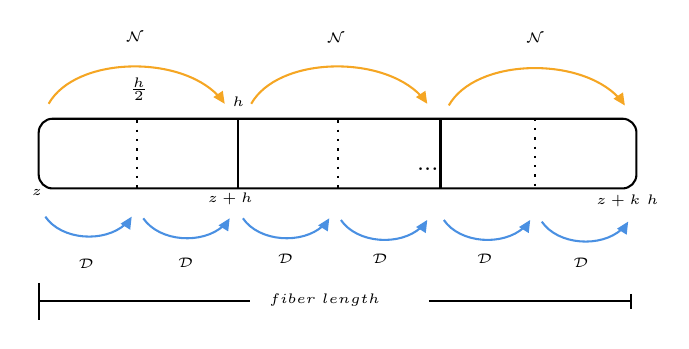
\begin{tikzpicture}[x=1.2pt,y=1.2pt,yscale=-1,xscale=1]
        %uncomment if require: \path (0,300); %set diagram left start at 0, and has height of 300
            
            %Rounded Rect [id:dp3852932235223505] 
            \draw   (100,115.2) .. controls (100,112.88) and (101.88,111) .. (104.2,111) -- (275.8,111) .. controls (278.12,111) and (280,112.88) .. (280,115.2) -- (280,127.8) .. controls (280,130.12) and (278.12,132) .. (275.8,132) -- (104.2,132) .. controls (101.88,132) and (100,130.12) .. (100,127.8) -- cycle ;
            %Straight Lines [id:da004144927883721339] 
            \draw    (160,111) -- (160,132) ;
            %Straight Lines [id:da3654232899891592] 
            \draw    (221,111) -- (221,132) ;
            %Straight Lines [id:da45475006001951823] 
            \draw    (100,166) -- (163.5,166) ;
            \draw [shift={(100,166)}, rotate = 180] [color={rgb, 255:red, 0; green, 0; blue, 0 }  ][line width=0.75]    (0,5.59) -- (0,-5.59)   ;
            %Straight Lines [id:da9346841303105087] 
            \draw    (217.5,166) -- (278.5,166) ;
            \draw [shift={(278.5,166)}, rotate = 180] [color={rgb, 255:red, 0; green, 0; blue, 0 }  ][line width=0.75]    (0,2.24) -- (0,-2.24)   ;
            %Curve Lines [id:da5361939697011324] 
            \draw [color={rgb, 255:red, 245; green, 166; blue, 35 }  ,draw opacity=1 ]   (103,106.5) .. controls (111.03,92.32) and (142.28,91.55) .. (154.14,104.16) ;
            \draw [shift={(156,106.5)}, rotate = 236.31] [fill={rgb, 255:red, 245; green, 166; blue, 35 }  ,fill opacity=1 ][line width=0.08]  [draw opacity=0] (3.57,-1.72) -- (0,0) -- (3.57,1.72) -- cycle    ;
            %Straight Lines [id:da41945250802592127] 
            \draw  [dash pattern={on 0.84pt off 2.51pt}]  (129.5,111.5) -- (129.5,132.5) ;
            %Straight Lines [id:da9865879096776455] 
            \draw  [dash pattern={on 0.84pt off 2.51pt}]  (190,111.5) -- (190,132.5) ;
            %Straight Lines [id:da5596453819308491] 
            \draw  [dash pattern={on 0.84pt off 2.51pt}]  (249.5,111) -- (249.5,132) ;
            %Curve Lines [id:da018780585468089805] 
            \draw [color={rgb, 255:red, 245; green, 166; blue, 35 }  ,draw opacity=1 ]   (164,106.5) .. controls (172.03,92.32) and (203.28,91.55) .. (215.14,104.16) ;
            \draw [shift={(217,106.5)}, rotate = 236.31] [fill={rgb, 255:red, 245; green, 166; blue, 35 }  ,fill opacity=1 ][line width=0.08]  [draw opacity=0] (3.57,-1.72) -- (0,0) -- (3.57,1.72) -- cycle    ;
            %Curve Lines [id:da8889794263264403] 
            \draw [color={rgb, 255:red, 245; green, 166; blue, 35 }  ,draw opacity=1 ]   (223.5,107) .. controls (231.53,92.82) and (262.78,92.05) .. (274.64,104.66) ;
            \draw [shift={(276.5,107)}, rotate = 236.31] [fill={rgb, 255:red, 245; green, 166; blue, 35 }  ,fill opacity=1 ][line width=0.08]  [draw opacity=0] (3.57,-1.72) -- (0,0) -- (3.57,1.72) -- cycle    ;
            %Curve Lines [id:da109759730738193] 
            \draw [color={rgb, 255:red, 74; green, 144; blue, 226 }  ,draw opacity=1 ]   (102,140.5) .. controls (106.92,147.66) and (119.86,148.41) .. (126.1,142.76) ;
            \draw [shift={(128,140.5)}, rotate = 482.01] [fill={rgb, 255:red, 74; green, 144; blue, 226 }  ,fill opacity=1 ][line width=0.08]  [draw opacity=0] (3.57,-1.72) -- (0,0) -- (3.57,1.72) -- cycle    ;
            %Curve Lines [id:da5801862642922446] 
            \draw [color={rgb, 255:red, 74; green, 144; blue, 226 }  ,draw opacity=1 ]   (131.5,141) .. controls (136.42,148.16) and (149.36,148.91) .. (155.6,143.26) ;
            \draw [shift={(157.5,141)}, rotate = 482.01] [fill={rgb, 255:red, 74; green, 144; blue, 226 }  ,fill opacity=1 ][line width=0.08]  [draw opacity=0] (3.57,-1.72) -- (0,0) -- (3.57,1.72) -- cycle    ;
            %Curve Lines [id:da32600514781734646] 
            \draw [color={rgb, 255:red, 74; green, 144; blue, 226 }  ,draw opacity=1 ]   (161.5,141) .. controls (166.42,148.16) and (179.36,148.91) .. (185.6,143.26) ;
            \draw [shift={(187.5,141)}, rotate = 482.01] [fill={rgb, 255:red, 74; green, 144; blue, 226 }  ,fill opacity=1 ][line width=0.08]  [draw opacity=0] (3.57,-1.72) -- (0,0) -- (3.57,1.72) -- cycle    ;
            %Curve Lines [id:da574569055792788] 
            \draw [color={rgb, 255:red, 74; green, 144; blue, 226 }  ,draw opacity=1 ]   (191,141.5) .. controls (195.92,148.66) and (208.86,149.41) .. (215.1,143.76) ;
            \draw [shift={(217,141.5)}, rotate = 482.01] [fill={rgb, 255:red, 74; green, 144; blue, 226 }  ,fill opacity=1 ][line width=0.08]  [draw opacity=0] (3.57,-1.72) -- (0,0) -- (3.57,1.72) -- cycle    ;
            %Curve Lines [id:da16955896501211276] 
            \draw [color={rgb, 255:red, 74; green, 144; blue, 226 }  ,draw opacity=1 ]   (222,141.5) .. controls (226.92,148.66) and (239.86,149.41) .. (246.1,143.76) ;
            \draw [shift={(248,141.5)}, rotate = 482.01] [fill={rgb, 255:red, 74; green, 144; blue, 226 }  ,fill opacity=1 ][line width=0.08]  [draw opacity=0] (3.57,-1.72) -- (0,0) -- (3.57,1.72) -- cycle    ;
            %Curve Lines [id:da7109799228168221] 
            \draw [color={rgb, 255:red, 74; green, 144; blue, 226 }  ,draw opacity=1 ]   (251.5,142) .. controls (256.42,149.16) and (269.36,149.91) .. (275.6,144.26) ;
            \draw [shift={(277.5,142)}, rotate = 482.01] [fill={rgb, 255:red, 74; green, 144; blue, 226 }  ,fill opacity=1 ][line width=0.08]  [draw opacity=0] (3.57,-1.72) -- (0,0) -- (3.57,1.72) -- cycle    ;
            
            % Text Node
            \draw (111,152.4) node [anchor=north west][inner sep=0.75pt]  [font=\tiny]  {$\mathcal{D}$};
            % Text Node
            \draw (141,151.9) node [anchor=north west][inner sep=0.75pt]  [font=\tiny]  {$\mathcal{D}$};
            % Text Node
            \draw (171,150.9) node [anchor=north west][inner sep=0.75pt]  [font=\tiny]  {$\mathcal{D}$};
            % Text Node
            \draw (199.5,150.9) node [anchor=north west][inner sep=0.75pt]  [font=\tiny]  {$\mathcal{D}$};
            % Text Node
            \draw (231,150.9) node [anchor=north west][inner sep=0.75pt]  [font=\tiny]  {$\mathcal{D}$};
            % Text Node
            \draw (260,151.9) node [anchor=north west][inner sep=0.75pt]  [font=\tiny]  {$\mathcal{D}$};
            % Text Node
            \draw (125.5,83.9) node [anchor=north west][inner sep=0.75pt]  [font=\tiny]  {$\mathcal{N}$};
            % Text Node
            \draw (186,84.4) node [anchor=north west][inner sep=0.75pt]  [font=\tiny]  {$\mathcal{N}$};
            % Text Node
            \draw (246,84.4) node [anchor=north west][inner sep=0.75pt]  [font=\tiny]  {$\mathcal{N}$};
            % Text Node
            \draw (97,131.4) node [anchor=north west][inner sep=0.75pt]  [font=\tiny]  {$z$};
            % Text Node
            \draw (150,132.4) node [anchor=north west][inner sep=0.75pt]  [font=\tiny]  {$z+h$};
            % Text Node
            \draw (267,132.9) node [anchor=north west][inner sep=0.75pt]  [font=\tiny]  {$z+k\ h$};
            % Text Node
            \draw (213,124.9) node [anchor=north west][inner sep=0.75pt]  [font=\small]  {$...$};
            % Text Node
            \draw (168.5,162.9) node [anchor=north west][inner sep=0.75pt]  [font=\tiny]  {$fiber\ length$};
            % Text Node
            \draw (126.5,97.9) node [anchor=north west][inner sep=0.75pt]  [font=\tiny]  {$\frac{h}{2}$};
            % Text Node
            \draw (157.5,103.4) node [anchor=north west][inner sep=0.75pt]  [font=\tiny]  {$h$};
            
                
            \end{tikzpicture}
        \end{figure}
        
%Write eq for propagation and explain LD vs LNL Bereiche ->  GVD only -> U(0,T) Gauss- und Sech-Pulse -> wie wird das Programm durchgeführt? Ergebnisse mithilfe Matplotlibs, und Darstelung in einer Web-App 